\documentclass[../../General.tex]{subfiles}
\begin{document}

\section{Antecedentes}

El panorama energético global se encuentra en una fase de transformación estructural con el objetivo de alcanzar el escenario de \textit{Net Zero Emissions} (NZE) para el año 2050. Dentro de este marco, se proyecta un crecimiento masivo de la demanda eléctrica global, fuertemente impulsada por la rápida electrificación de usos finales que anteriormente dependían de combustibles fósiles, destacando especialmente la industria y el transporte \citep{IEA_NZE_2021}. Para cubrir esta acelerada demanda eléctrica sin incrementar las emisiones, las energías limpias asumen un rol indispensable; específicamente, la energía solar fotovoltaica y la eólica deben cuadruplicar su ritmo de despliegue histórico, requiriendo alcanzar adiciones anuales de 630 GW de energía solar y 390 GW de energía eólica para el año 2030 \citep{IEA_NZE_2021}. 

De acuerdo con la hoja de ruta de la Agencia Internacional de Energía (IEA), este escenario marca el inicio de una era dominada por las energías limpias, donde el consumo eléctrico escala mientras que el suministro de energía primaria proveniente de combustibles fósiles cae del 80\,\% en 2020 a poco más del 20\,\% en 2050 (Véase Figura \ref{fig:TendenciasNZE2050}). A pesar de que la energía solar y eólica se convierten en los pilares del sistema, la inversión anual en energía limpia debe aumentar desde los niveles actuales hasta alcanzar los 4 billones de dólares para 2030 \citep{IEA_NZE_2021}. Esta transición requiere superar cuellos de botella críticos, especialmente en la expansión y modernización de las redes eléctricas, cuya inversión anual debe duplicarse para evitar deficiencias en el balance energético y asegurar la integración de la generación variable, minimizando así el desperdicio forzado de energía limpia \citep{IEA_WEO_2025}.

\begin{figure}[H]
	% Fuerza la alineación izquierda y quita los ":" después del número
	\captionsetup{justification=raggedright, singlelinecheck=false, labelsep=none}
	
	\caption[Tendencias de la demanda energética proyectadas al 2050 bajo el escenario de Net Zero Emissions.]{} 
	
	% Vspace negativo opcional para acercar el texto cursivo al número de figura
	\textit{Tendencias de la demanda energética proyectadas al 2050 bajo el escenario de Net Zero Emissions.} \par\medskip
	
	\centering
	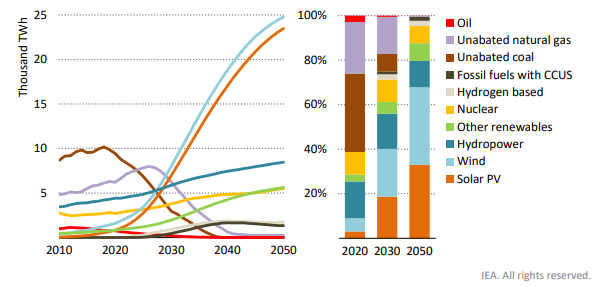
\includegraphics[width=0.8\textwidth]{Recursos/Imagenes/Graficas/NZE2050.png} \par\medskip
	
	\raggedright
	\footnotesize \textit{Nota.} Gráfico adaptado del reporte Net Zero Emissions by 2050 \citep{IEA_NZE_2021}.
	\label{fig:TendenciasNZE2050}
\end{figure}



En el ámbito nacional, la demanda energética peruana crece a un ritmo promedio anual de entre 3\,\% y 3.5\,\%, aunque con una profunda disparidad regional que contrasta el incremento del 26\,\% en la zona centro con severas contracciones en el norte (36\,\%) y sur (-18\,\%) \citep{ICEX2025}. En paralelo, la matriz de producción eléctrica, que alcanzó los 60 GW en 2024, avanza en su transición hacia fuentes limpias \citep{ProActivo2025}. Muestra de ello es que, para octubre de 2025, la generación mediante recursos renovables no convencionales (solar, eólica, bagazo y biogás) experimentó un crecimiento interanual del 27\,\%, representando el 13\,\% del total producido, en línea con el objetivo estratégico del Estado de alcanzar una participación del 20\,\% para el año 2030.

Las nuevas tendencias energéticas, lideradas por la tecnología solar fotovoltaica, plantean retos técnicos complejos para garantizar la eficiencia operativa \citep{XPower2024}. A medida que los proyectos fotovoltaicos escalan y se sitúan en terrenos topográficamente irregulares, factores como la variabilidad espacial de la irradiancia, las fluctuaciones térmicas, la suciedad y el ensombrecimiento afectan directamente la producción \citep{Salinas2025}. Bajo este escenario, la instrumentación rigurosa se convierte en un componente crítico. El despliegue estratégico de redes de sensores, equipos de diagnóstico y plataformas de monitoreo continuo es indispensable para determinar el índice de rendimiento (\textit{Performance Ratio}) bajo normativas como la IEC 61724 \citep{IEC61724-1_2021}. Esta precisión no solo es necesaria para validar el diseño de la planta frente a la variabilidad climática, sino que habilita estrategias de mantenimiento predictivo capaces de anticipar anomalías, minimizar tiempos de inactividad y asegurar el retorno de inversión, consolidando a la energía solar como una infraestructura económica y resiliente \citep{Anatrac}.

Sin embargo, para sostener este volumen de expansión, la industria solar se enfrenta a nuevas y complejas realidades geográficas para el emplazamiento de sus proyectos. Un número cada vez mayor de plantas fotovoltaicas a gran escala experimenta una transición hacia terrenos con topografía compleja y áreas montañosas, lo que genera una distribución espacial altamente fragmentada en el terreno \citep{Mao2025}.Esta nueva realidad montañosa cambia por completo cómo se comporta el viento en el lugar; las laderas actúan como una gran barrera física que frena y atrapa el aire en la parte más baja del terreno, mientras que hace que el viento acelere y sople con fuerza al llegar a la cima \citep{Xu2024}. Estas variaciones extremas en la velocidad del viento afectan directamente la enfriamiento de los paneles a lo largo del terreno, creando zonas con niveles de temperatura muy desiguales en la planta. 
La convergencia de estos flujos de aire irregulares, la alteración en la altura respecto al suelo y los patrones de sombras no uniformes crean un mosaico de microclimas muy distintos a lo largo de la instalación \citep{Armstrong2026}. En consecuencia, surge la necesidad ineludible de contar con herramientas dinámicas de diagnóstico que sean capaces de mapear estas variaciones espaciales del terreno, un desafío crítico que la instrumentación estática convencional es físicamente incapaz de resolver.

\end{document}

